To quantify the effectiveness of this method we compare it to the existing OpenDataCam tool.
We will compare the counts, produced by OpenDataCam and manual annotation, of cyclists at strategic parts of the intersection with the counts produced by our system. The manually annotated counts being the ground truth.
This is followed by an analysis of the desire paths and an analysis of body language when cyclist trigger a defined
alert zone.
\ \\ 

\subsubsection{Comparison between three different methods}
Table x shows a comparison between OpenDataCam, manual annotation and our method.
The comparison is based on how well each method captured cyclist driving on along three different 
desire lines towards Fisketorvet.
Our method captured x ‰ of what manual annotation has, manual annotation being the base line.
\ \\

\subsubsection{Interpretation of desire paths desire paths}
The trajectory analysis in Figure~\ref{Rainbow} we can determine eight commonly taken desire paths. 
Where as with manual annotation we can determine x amount.
\ \\
\raggedbottom
\ \\ 
\noindent
\begin{tabular}{@{}cc}
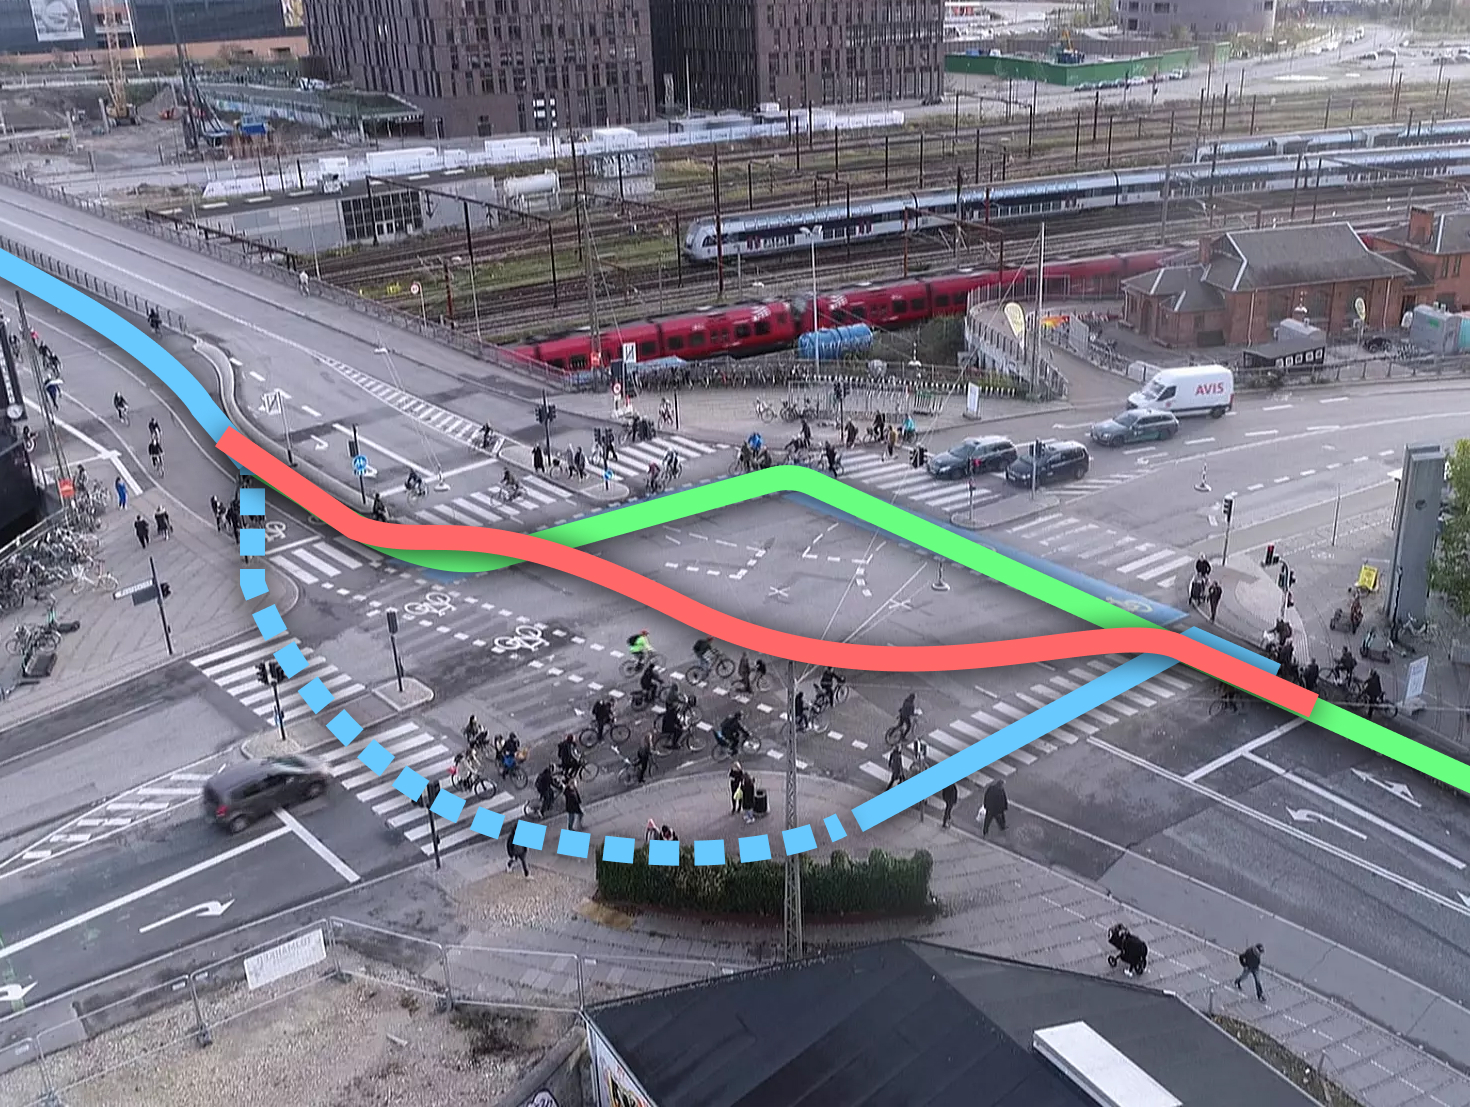
\includegraphics[width=1.0\columnwidth]{paths} 
\end{tabular}
\captionof{figure}{Common trajectories of cyclists comming from NW}
\label{traject}

\ \\
\subsubsection{behavioral analysis}
The marking of alert zones works well and allows the analysis of cyclist when encountering marked sections of the 
intersection. In Figure~\ref{Alert} we can see by the facial expressions 
\ \\
\raggedbottom
\ \\ 
\noindent
\begin{tabular}{@{}cc}
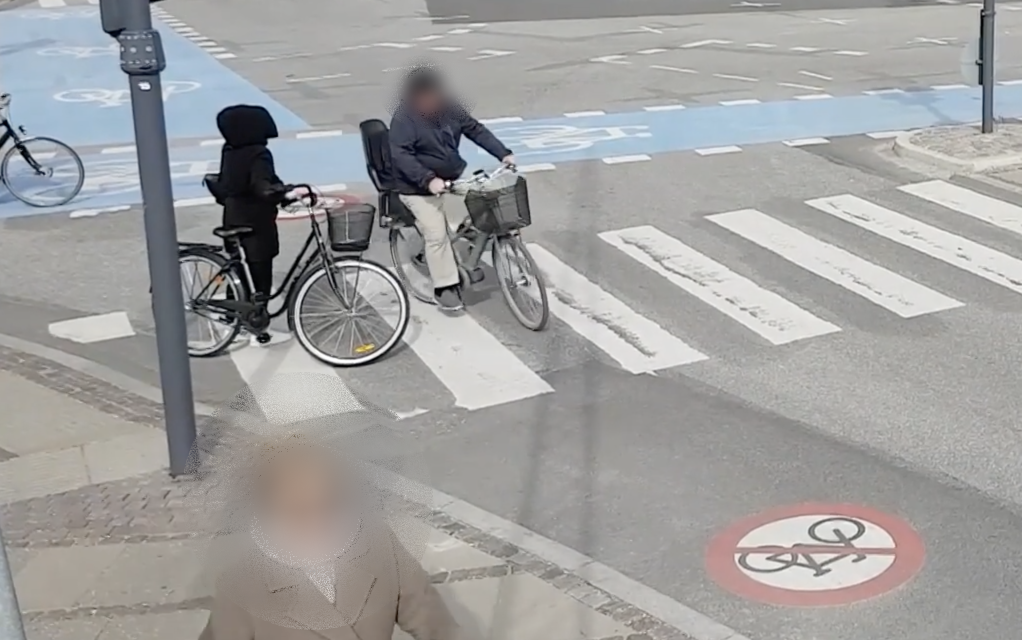
\includegraphics[width=1.0\columnwidth]{abnormal_blur.png} 
\end{tabular}
\captionof{figure}{Alert zone triggered}
\label{Alert}
\ \\

% Which are all compared to the "ground truth" dataset that we annotate manually. We know from previous works with OpenDataCam
% that vehicle detection has achieved 95\% accuracy while performing worse for pedestrians and motorcycles (\cite{BROEKMAN2021100068}).

Another commonly observed behaviour was cyclists who tried to shorten the trajectories of their turns.
This was common
